% This file was created with matplot2tikz v0.5.1.
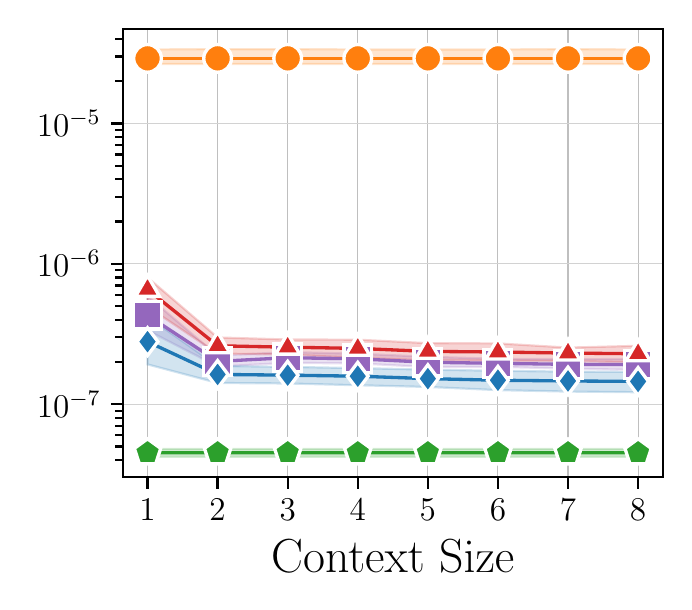
\begin{tikzpicture}

\definecolor{crimson2143940}{RGB}{214,39,40}
\definecolor{darkgray}{RGB}{169,169,169}
\definecolor{darkorange25512714}{RGB}{255,127,14}
\definecolor{darkslategray38}{RGB}{38,38,38}
\definecolor{forestgreen4416044}{RGB}{44,160,44}
\definecolor{lightgray204}{RGB}{204,204,204}
\definecolor{mediumpurple148103189}{RGB}{148,103,189}
\definecolor{steelblue31119180}{RGB}{31,119,180}

\begin{axis}[
    line width=0.8pt,             % Thicker axis outline
    axis line style={black},      % Solid black contrast
    log basis y={10},
    tick align=outside,
    % title={Sheet Deformation},
    xlabel={Context Size},
    xlabel style={font=\LARGE, color=black},
    % ylabel={Full Rollout MSE},
    ylabel style={font=\LARGE, color=black},
    tick label style={font=\large, color=black},
    xmajorgrids,
    xtick={1,2,3,4,5,6,7,8},           % Specify tick positions
    xticklabels={1,2,3,4,5,6,7,8},     % Specify tick labels
    xmajorticks=true,                  % Ensure ticks are enabled
    xtick pos=bottom,
    xmin=0.65, xmax=8.35,
    xtick style={color=black, line width=0.8pt},
    y grid style={lightgray!70},  % Darker grid lines
    ymajorgrids,
    % Kept your original y-range for Sheet Deformation
    ymin=3.02647033233786e-08, ymax=4.72304384868436e-05,
    ymode=log,
    ytick pos=left,
    ytick style={color=black, line width=0.8pt}
]
\path [draw=darkorange25512714, fill=darkorange25512714, opacity=0.2]
(axis cs:1,3.36614743901009e-05)
--(axis cs:1,2.65160761045991e-05)
--(axis cs:2,2.65160633716732e-05)
--(axis cs:3,2.65160815615673e-05)
--(axis cs:4,2.65160651906626e-05)
--(axis cs:5,2.65160842900514e-05)
--(axis cs:6,2.65160651906626e-05)
--(axis cs:7,2.65160615526838e-05)
--(axis cs:8,2.65160770140938e-05)
--(axis cs:8,3.36613748004311e-05)
--(axis cs:8,3.36613748004311e-05)
--(axis cs:7,3.3812106721598e-05)
--(axis cs:6,3.36614189109241e-05)
--(axis cs:5,3.36613820763887e-05)
--(axis cs:4,3.36651707698365e-05)
--(axis cs:3,3.3812126275734e-05)
--(axis cs:2,3.38121380991652e-05)
--(axis cs:1,3.36614743901009e-05)
--cycle;
\path [draw=mediumpurple148103189, fill=mediumpurple148103189, opacity=0.2]
(axis cs:1,5.88738842566272e-07)
--(axis cs:1,3.35676525331508e-07)
--(axis cs:2,1.85870671742805e-07)
--(axis cs:3,1.96925267204051e-07)
--(axis cs:4,1.95514850531708e-07)
--(axis cs:5,1.83973703826723e-07)
--(axis cs:6,1.84667015901141e-07)
--(axis cs:7,1.79375916786739e-07)
--(axis cs:8,1.75611702957212e-07)
--(axis cs:8,2.09818125540551e-07)
--(axis cs:8,2.09818125540551e-07)
--(axis cs:7,2.0945153522689e-07)
--(axis cs:6,2.10796272881453e-07)
--(axis cs:5,2.17816499059609e-07)
--(axis cs:4,2.29190582956562e-07)
--(axis cs:3,2.35318907471083e-07)
--(axis cs:2,2.2199241556109e-07)
--(axis cs:1,5.88738842566272e-07)
--cycle;
\path [draw=crimson2143940, fill=crimson2143940, opacity=0.2]
(axis cs:1,7.99657911443319e-07)
--(axis cs:1,4.95366769825978e-07)
--(axis cs:2,2.29571838872289e-07)
--(axis cs:3,2.2567823521058e-07)
--(axis cs:4,2.14074685089827e-07)
--(axis cs:5,2.05354318438822e-07)
--(axis cs:6,2.04547085047579e-07)
--(axis cs:7,2.02685072281383e-07)
--(axis cs:8,1.99070296247328e-07)
--(axis cs:8,2.60654125838755e-07)
--(axis cs:8,2.60654125838755e-07)
--(axis cs:7,2.5319228313947e-07)
--(axis cs:6,2.71147559516294e-07)
--(axis cs:5,2.72206335694136e-07)
--(axis cs:4,2.88310805807157e-07)
--(axis cs:3,2.89073540216123e-07)
--(axis cs:2,2.99039442097637e-07)
--(axis cs:1,7.99657911443319e-07)
--cycle;
\path [draw=forestgreen4416044, fill=forestgreen4416044, opacity=0.2]
(axis cs:1,4.80712571970798e-08)
--(axis cs:1,4.22752091111533e-08)
--(axis cs:2,4.22765928931312e-08)
--(axis cs:3,4.22761168294983e-08)
--(axis cs:4,4.22756762930021e-08)
--(axis cs:5,4.22754737883224e-08)
--(axis cs:6,4.22760813023615e-08)
--(axis cs:7,4.22762393981202e-08)
--(axis cs:8,4.22761363694235e-08)
--(axis cs:8,4.80717456952107e-08)
--(axis cs:8,4.80717456952107e-08)
--(axis cs:7,4.80716195738751e-08)
--(axis cs:6,4.80715307560331e-08)
--(axis cs:5,4.80718487239074e-08)
--(axis cs:4,4.80715627304562e-08)
--(axis cs:3,4.80713300277102e-08)
--(axis cs:2,4.80721435991427e-08)
--(axis cs:1,4.80712571970798e-08)
--cycle;
\path [draw=steelblue31119180, fill=steelblue31119180, opacity=0.2]
(axis cs:1,4.2036381842081e-07)
--(axis cs:1,1.9226405356676e-07)
--(axis cs:2,1.41688168753262e-07)
--(axis cs:3,1.40581622787295e-07)
--(axis cs:4,1.36576154829982e-07)
--(axis cs:5,1.32790113127612e-07)
--(axis cs:6,1.26062680294581e-07)
--(axis cs:7,1.23081605352127e-07)
--(axis cs:8,1.21796588814505e-07)
--(axis cs:8,1.69823117346368e-07)
--(axis cs:8,1.69823117346368e-07)
--(axis cs:7,1.70735770410602e-07)
--(axis cs:6,1.73041364348592e-07)
--(axis cs:5,1.76507832350126e-07)
--(axis cs:4,1.80823377604611e-07)
--(axis cs:3,1.84580066786566e-07)
--(axis cs:2,1.87385303718202e-07)
--(axis cs:1,4.2036381842081e-07)
--cycle;
\addplot [very thick, darkorange25512714, mark=*, mark size=5, mark options={solid,draw=white}]
table {%
1 2.90772063635814e-05
2 2.90771795334877e-05
3 2.90771822619718e-05
4 2.90771881736873e-05
5 2.90771822619718e-05
6 2.90771863546979e-05
7 2.90771654363198e-05
8 2.90771749860141e-05
};
\addplot [very thick, mediumpurple148103189, mark=square*, mark size=5, mark options={solid,draw=white}]
table {%
1 4.29895926856716e-07
2 2.01897488949498e-07
3 2.14529986664047e-07
4 2.10535318956317e-07
5 1.99196005468139e-07
6 1.95524226143107e-07
7 1.92447579649979e-07
8 1.91391933412888e-07
};
\addplot [very thick, crimson2143940, mark=triangle*, mark size=5, mark options={solid,draw=white}]
table {%
1 6.56739722160182e-07
2 2.60814303487678e-07
3 2.54909295449579e-07
4 2.49815663266872e-07
5 2.37835159566657e-07
6 2.35567323869645e-07
7 2.31347954127159e-07
8 2.28905921773048e-07
};
\addplot [very thick, forestgreen4416044, mark=pentagon*, mark size=5, mark options={solid,draw=white}]
table {%
1 4.51732331541166e-08
2 4.5174368246137e-08
3 4.51737234286043e-08
4 4.51736195117292e-08
5 4.51736612561149e-08
6 4.51738060291973e-08
7 4.51739294859976e-08
8 4.51739410323171e-08
};
\addplot [very thick, steelblue31119180, mark=diamond*, mark size=5, mark options={solid,draw=white}]
table {%
1 2.79103588241014e-07
2 1.63104733275077e-07
3 1.61079679372733e-07
4 1.58422608365072e-07
5 1.52170954947906e-07
6 1.48282151002377e-07
7 1.46461310635004e-07
8 1.45410574248217e-07
};
\end{axis}

\end{tikzpicture}
